\documentclass[a4paper,12pt]{article}

% ---------------- PACOTES ----------------
\usepackage[utf8]{inputenc}
\usepackage[T1]{fontenc}
\usepackage[brazil]{babel}
\usepackage{geometry}
\usepackage{graphicx}
\usepackage{amsmath, amssymb}
\usepackage{siunitx}
\usepackage{caption}
\usepackage{subcaption}
\usepackage{float}
\usepackage{indentfirst}
\usepackage{hyperref}
\usepackage{array}

\geometry{margin=2.5cm}

% ---------------- INÍCIO ----------------
\begin{document}

% -------- CAPA --------
\begin{titlepage}

    % Logo
    \noindent
    \begin{minipage}[c]{0.18\textwidth}
        \includegraphics[width=\linewidth]{png-logo-ufma-colorido.png}
        \end{minipage}
    \hfill
    \begin{minipage}[c]{0.78\textwidth}
    \raggedright
    {\small \textbf{UNIVERSIDADE FEDERAL DO MARANHÃO - UFMA\\
    CENTRO DE CIÊNCIA EXATAS E TECNOLOGIA - CCET\\
    ENGENHARIA DA COMPUTAÇÃO - EECP\\
    ARQUITETURA DE COMPUTADORES
    }}
    \end{minipage}

    \vspace{2cm}

    % Título
    \begin{center}
    {\Large \textbf{Sistema Embarcado de Monitoramento Ambiental e Meteorológico}}
    \end{center}

    \vspace{2cm}

    % Discentes
    \begin{center}
    {\large Discentes:\\
    \large \textbf{}\\
    \large \textbf{João Henrique Calixto Teixeira (2023030390)}\\
    \large \textbf{Marcos Paulo Dominice Silva (2023030318)}\\
    \large \textbf{Rai Abreu Machado (2023034498)}\\
    \large \textbf{Ronald Loureiro Camara (2023034460)}\\
    \large \textbf{Wesley Ferreira Costa (2023034442)}}\\
    \end{center}

    \vspace{1.5cm}

    % Docente
    \begin{center}
    {\large Docente:\\
    \textbf{Luiz Henrique Neves Rodrigues}}
    \end{center}

    \vfill

    % Rodapé
    \begin{center}
    {\large \textbf{São Luís - MA}}\\
    {\large \textbf{2026}}
    \end{center}

\end{titlepage}

% -------- SUMÁRIO --------
\tableofcontents
\newpage
% -------- SEÇÕES --------

\section{Cronograma}

O desenvolvimento do projeto foi realizado conforme o cronograma apresentado a seguir, contemplando as etapas de estudo teórico, planejamento da arquitetura do sistema, integração dos sensores, desenvolvimento do firmware, coleta experimental dos dados e elaboração da documentação técnica.

\vspace{0.5cm}
\textbf{Abril}
\begin{itemize}
\item 22/04 (Qua) -- Estudo teórico da arquitetura do microcontrolador ATmega328P.
\item 27/04 (Seg) -- Continuação do estudo teórico.
\item 29/04 (Qua) -- Definição dos protocolos de comunicação do projeto.
\end{itemize}

\textbf{Maio}
\begin{itemize}
\item 04/05 (Seg) -- Planejamento do circuito eletrônico.
\item 06/05 (Qua) -- Início da montagem em protoboard.
\item 11/05 (Seg) -- Integração inicial dos sensores.
\item 13/05 (Qua) -- Continuação da integração dos sensores.
\item 18/05 (Seg) -- Desenvolvimento do firmware embarcado.
\item 20/05 (Qua) -- Implementação das leituras dos sensores e testes iniciais.
\item 25/05 (Seg) -- Ajustes e correções no sistema.
\item 27/05 (Qua) -- Validação funcional da arquitetura implementada.
\end{itemize}

\textbf{Junho}
\begin{itemize}
\item 01/06 (Seg) -- Coleta de dados experimentais.
\item 03/06 (Qua) -- Continuação da coleta de dados.
\item 08/06 (Seg) -- Organização e tratamento dos dados obtidos.
\item 10/06 (Qua) -- Análise dos resultados experimentais.
\item 15/06 (Seg) -- Ajustes finais no sistema embarcado.
\item 17/06 (Qua) -- Elaboração do relatório técnico final.
\item 22/06 (Seg) -- Apresentação final do projeto.
\end{itemize}

A Figura \ref{fig:gantt} apresenta o gráfico de Gantt elaborado para acompanhamento das etapas de desenvolvimento do projeto, permitindo visualizar a distribuição temporal das atividades executadas ao longo do período de realização.

\begin{figure}[H]
\centering
\includegraphics[width=0.9\linewidth]{gantt.jpeg}
\caption{Gráfico de Gantt do cronograma de desenvolvimento do projeto}
\label{fig:gantt}
\end{figure}

\section{Materiais e Metodologia}

\subsection{Materiais}

\begin{enumerate}

    \item \textbf{Arduino Nano} -- Plataforma de desenvolvimento baseada no microcontrolador ATmega328P, responsável pelo processamento dos dados, gerenciamento dos sensores e execução do firmware do sistema embarcado.
    
    \item \textbf{Protoboard} -- Placa de prototipagem utilizada para montagem do circuito eletrônico sem a necessidade de soldagem, permitindo conexões rápidas entre os componentes do sistema.
    
    \item \textbf{Sensor BME280} -- Sensor digital utilizado para medição de temperatura, umidade relativa do ar e pressão atmosférica, além da estimativa aproximada de altitude.
    
    \item \textbf{Sensor BH1750} -- Sensor digital utilizado para medição da intensidade luminosa ambiente em lux.
    
    \item \textbf{Sensor MQ-135} -- Sensor analógico utilizado para monitoramento relativo da qualidade do ar através da detecção de gases e compostos voláteis presentes no ambiente.
    
    \item \textbf{Jumpers} -- Fios condutores utilizados para realizar as conexões elétricas entre o Arduino Nano, sensores e protoboard.
    
    \item \textbf{Cabo USB} -- Utilizado para alimentação do Arduino Nano e comunicação serial com o computador durante a programação e monitoramento dos dados.
    
    \item \textbf{Computador} -- Equipamento utilizado para desenvolvimento do firmware, gravação do código no microcontrolador e visualização dos dados através do Monitor Serial da IDE Arduino.
    
    \item \textbf{IDE Arduino} -- Ambiente de desenvolvimento utilizado para escrita, compilação e upload do firmware para o microcontrolador ATmega328P.
    
\end{enumerate}

\subsection{Metodologia}

Inicialmente, foi realizada a montagem do circuito eletrônico em protoboard, integrando os sensores BME280, BH1750 e MQ-135 ao sistema embarcado.

Os sensores BME280 e BH1750 foram conectados utilizando o protocolo de comunicação I2C, compartilhando as linhas SDA e SCL do microcontrolador. Já o sensor MQ-135 foi integrado através de sua saída analógica, conectada ao pino A0 para utilização do conversor analógico-digital (ADC).

A Tabela \ref{tab:bme280} apresenta as conexões utilizadas no sensor BME280.

\begin{table}[H]
\centering
\caption{Conexões do sensor BME280}
\label{tab:bme280}
\begin{tabular}{|c|c|}
\hline
\textbf{BME280} & \textbf{Conexão} \\ \hline
VIN & 3V3 \\ \hline
GND & GND \\ \hline
SDA & A4 \\ \hline
SCL & A5 \\ \hline
\end{tabular}
\end{table}

A Tabela \ref{tab:bh1750} apresenta as conexões utilizadas no sensor BH1750.

\begin{table}[H]
\centering
\caption{Conexões do sensor BH1750}
\label{tab:bh1750}
\begin{tabular}{|c|c|}
\hline
\textbf{BH1750} & \textbf{Conexão} \\ \hline
VCC & 3V3 \\ \hline
GND & GND \\ \hline
SDA & A4 \\ \hline
SCL & A5 \\ \hline
ADDR & GND \\ \hline
\end{tabular}
\end{table}

Para realizar essa comunicação, o ATmega328P possui internamente um módulo de hardware dedicado denominado TWI (\textit{Two Wire Interface}). A interface TWI é a implementação desenvolvida pela Atmel para comunicação compatível com o protocolo I2C.

A utilização do termo TWI ocorre porque a nomenclatura ``I2C'' é registrada pela Philips, fazendo com que outros fabricantes utilizem nomes alternativos para tecnologias compatíveis. Apesar disso, o funcionamento da TWI do ATmega328P é totalmente compatível com dispositivos I2C utilizados no projeto.

Internamente, a interface TWI do ATmega328P é composta por circuitos digitais responsáveis pelo gerenciamento automático da comunicação serial entre o microcontrolador e os sensores conectados ao barramento. Entre suas principais funções estão:

\begin{itemize}
\item geração do sinal de clock da comunicação;
\item envio e recebimento serial de dados;
\item sincronização entre dispositivos conectados;
\item detecção e reconhecimento de endereços I2C;
\item controle dos sinais de início (\textit{Start}) e parada (\textit{Stop});
\item armazenamento temporário dos dados recebidos;
\item controle do fluxo de transmissão através de registradores internos.
\end{itemize}

O funcionamento da TWI ocorre através de registradores internos específicos do ATmega328P, responsáveis pelo controle da transmissão de dados. Durante a comunicação, o microcontrolador envia o endereço do dispositivo desejado pelo barramento I2C. Caso o endereço corresponda ao sensor conectado, o dispositivo responde ao ATmega328P e inicia a troca de informações.

No sistema desenvolvido, o ATmega328P atua como dispositivo mestre (\textit{Master}), sendo responsável por iniciar toda a comunicação. Os sensores BME280 e BH1750 atuam como dispositivos escravos (\textit{Slave}), respondendo às solicitações enviadas pelo microcontrolador através de seus respectivos endereços I2C.

A biblioteca \texttt{Wire.h}, utilizada no firmware do projeto, realiza a interface entre o código desenvolvido em linguagem C++ e o módulo TWI interno do ATmega328P. Dessa forma, funções de alto nível podem ser utilizadas para transmissão e recepção de dados sem necessidade de manipular diretamente os registradores do microcontrolador.

No contexto do sistema embarcado desenvolvido, a interface TWI possui papel fundamental na aquisição dos dados ambientais, permitindo que o ATmega328P obtenha informações digitais de temperatura, umidade, pressão atmosférica e luminosidade de maneira rápida, organizada e eficiente.

Além disso, o uso do barramento I2C através da interface TWI reduz significativamente a quantidade de conexões elétricas necessárias no circuito, aumentando a organização da montagem, reduzindo a complexidade do hardware e facilitando futuras expansões do sistema com novos sensores digitais.

O sensor MQ-135 foi conectado conforme apresentado na Tabela \ref{tab:mq135}.

\begin{table}[H]
\centering
\caption{Conexões do sensor MQ-135}
\label{tab:mq135}
\begin{tabular}{|c|c|}
\hline
\textbf{MQ-135} & \textbf{Conexão} \\ \hline
VCC & 5V \\ \hline
GND & GND \\ \hline
AO & A0 \\ \hline
\end{tabular}
\end{table}

Após a montagem física do circuito, foi desenvolvido o firmware responsável pela inicialização dos sensores, aquisição dos dados ambientais, processamento das informações e exibição dos resultados no Monitor Serial.

Além da montagem em protoboard, foi elaborado um esquemático eletrônico utilizando o software KiCad, permitindo representar de forma organizada todas as conexões elétricas do sistema embarcado desenvolvido.

A Figura \ref{fig} apresenta o esquemático completo do circuito implementado no projeto.

\begin{figure}[H]
\centering
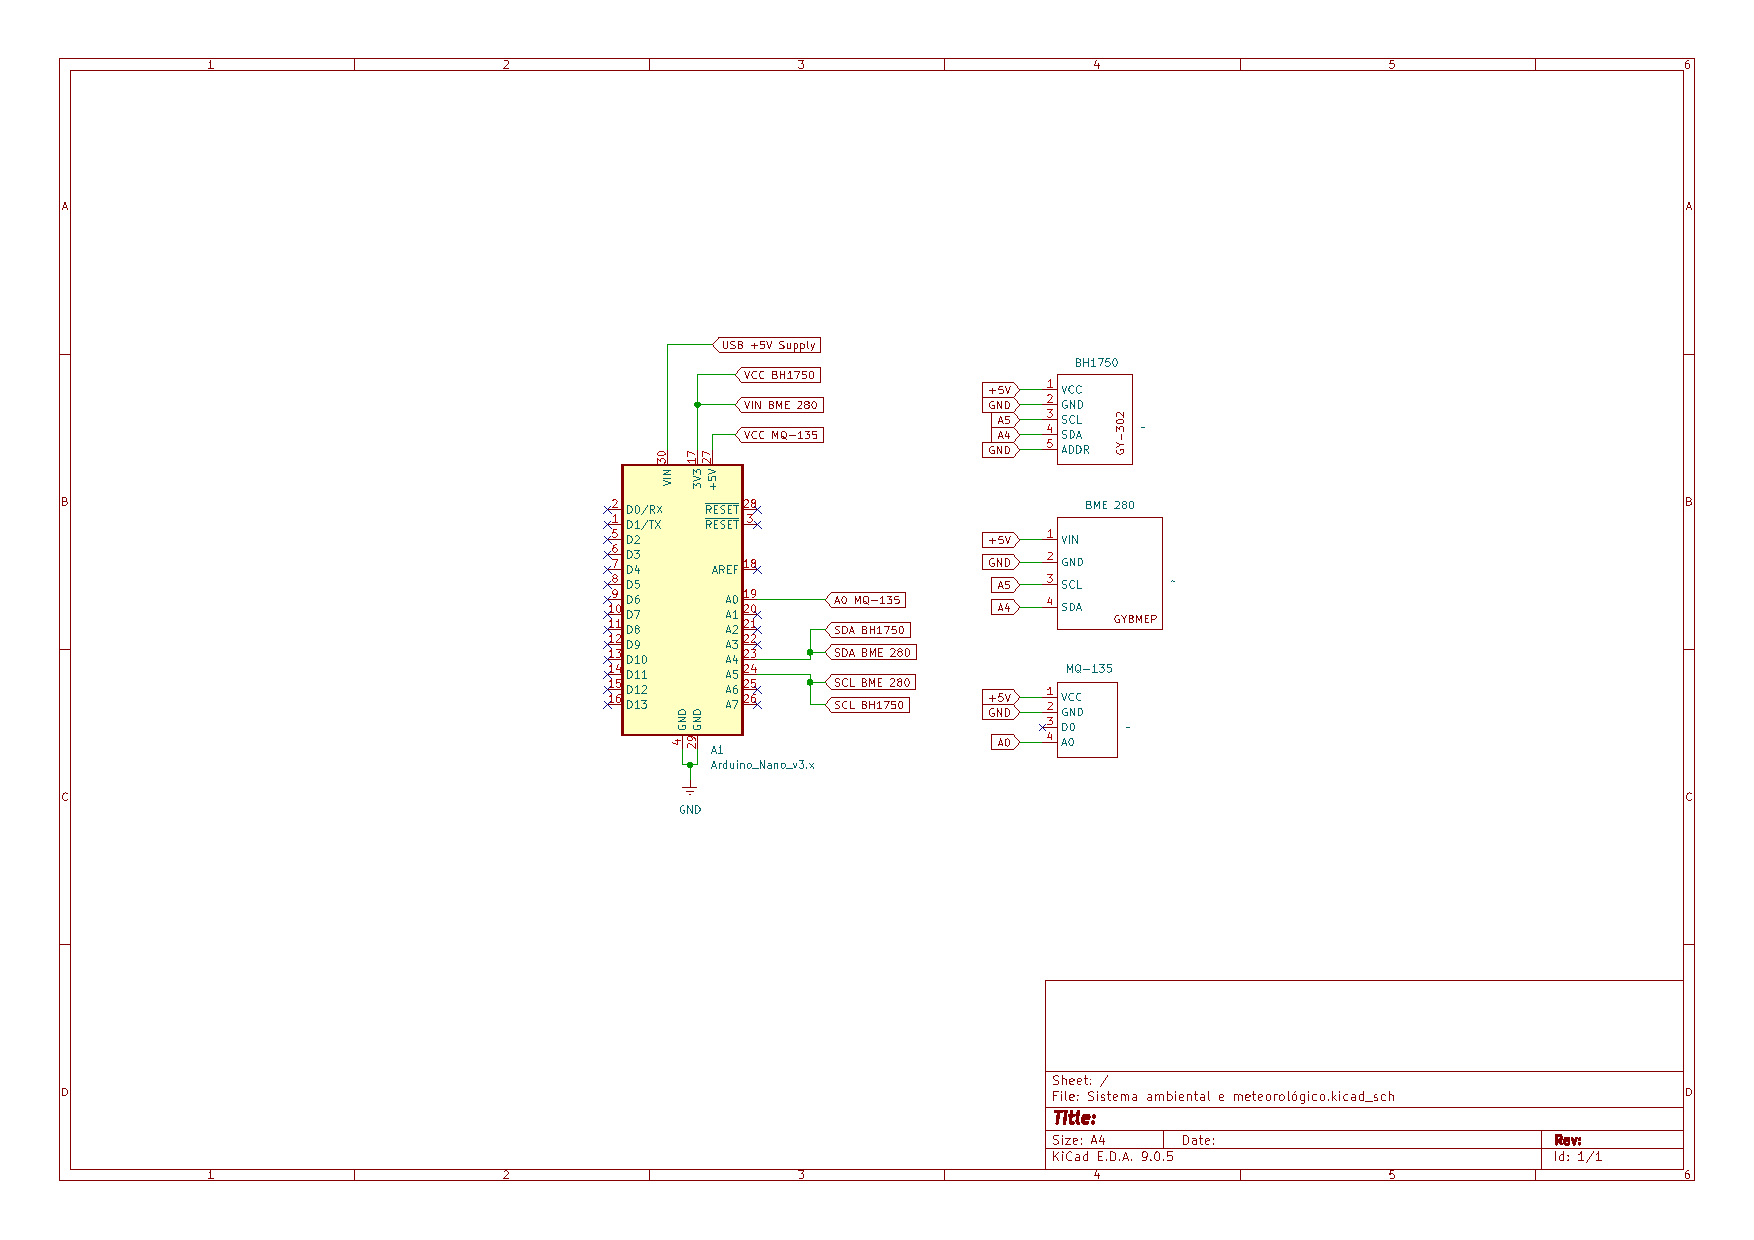
\includegraphics[width=0.9\linewidth]{Esquematico sistema ambiental e meteorológico.pdf}
\caption{Esquemático eletrônico do sistema de monitoramento ambiental desenvolvido no KiCad}
\label{fig}
\end{figure}

Para comunicação com os sensores digitais, foram utilizadas as bibliotecas:
\begin{itemize}
    \item \texttt{Wire.h};
    \item \texttt{Adafruit\_Sensor.h};
    \item \texttt{Adafruit\_BME280.h};
    \item \texttt{BH1750.h}.
\end{itemize}

O sensor BME280 foi inicializado utilizando o endereço I2C \texttt{0x76}, enquanto o BH1750 operou utilizando seu endereço padrão \texttt{0x23}.

Durante a execução do firmware, o sistema realiza leituras periódicas de:
\begin{itemize}
    \item temperatura;
    \item umidade relativa do ar;
    \item pressão atmosférica;
    \item altitude aproximada;
    \item luminosidade ambiente;
    \item qualidade relativa do ar.
\end{itemize}

A leitura do sensor MQ-135 foi realizada através da função:

\begin{verbatim}
analogRead(MQ135_PIN);
\end{verbatim}

O sensor MQ-135 fornece em sua saída um sinal analógico proporcional à concentração dos gases presentes no ambiente. Essa tensão analógica é aplicada ao pino A0 do Arduino Nano, sendo posteriormente interpretada pelo conversor analógico-digital (ADC) interno do microcontrolador ATmega328P.

O ADC do ATmega328P possui resolução de 10 bits, permitindo converter tensões analógicas em valores digitais compreendidos entre 0 e 1023. Internamente, o conversor realiza amostragens da tensão presente na entrada analógica e compara esse valor com uma tensão de referência previamente definida pelo sistema.

O processo de conversão ocorre de forma sequencial, no qual o ADC transforma o nível contínuo de tensão em uma representação binária equivalente. Dessa forma, sinais analógicos provenientes do sensor MQ-135 podem ser processados digitalmente pelo microcontrolador.

Além disso, o ATmega328P utiliza um multiplexador analógico interno (MUX), responsável por selecionar qual entrada analógica será encaminhada ao conversor ADC. No projeto desenvolvido, o canal correspondente ao pino A0 foi utilizado para aquisição do sinal proveniente do MQ-135.

A Figura \ref{fig:adc} ilustra o princípio básico de funcionamento da conversão analógico-digital realizada pelo ADC do microcontrolador.

\begin{figure}[H]
    \centering
    \includegraphics[width=0.9\linewidth]{adc.jpg}
    \caption{Processo de conversão analógico-digital realizado pelo ADC do ATmega328P}
    \label{fig:adc}
\end{figure}

Após a conversão analógico-digital, o firmware realiza o processamento matemático do sinal obtido pelo sensor MQ-135. Inicialmente, o valor digital retornado pelo ADC é convertido em tensão elétrica. Em seguida, o sistema calcula a resistência variável interna do sensor e aplica a curva característica do MQ-135 para estimativa aproximada da concentração de gases em PPM (\textit{Parts Per Million}).

Com base no valor calculado em PPM, o firmware executa uma lógica condicional responsável pela classificação da qualidade do ar conforme os limites estabelecidos no código.

A Tabela \ref{tab:qualidade_ar} apresenta os níveis utilizados no sistema.

\begin{table}[H]
\centering
\caption{Classificação da qualidade do ar em PPM}
\label{tab:qualidade_ar}
\begin{tabular}{|c|c|}
\hline
\textbf{Faixa (PPM)} & \textbf{Classificação} \\ \hline
0 -- 450 & Excelente \\ \hline
451 -- 1000 & Adequada \\ \hline
1001 -- 1500 & Ruim \\ \hline
Acima de 1500 & Crítica \\ \hline
\end{tabular}
\end{table}

Dessa forma, o sistema embarcado realiza todo o processo de aquisição, conversão, processamento e classificação da qualidade do ar em tempo real, permitindo monitorar continuamente as condições ambientais do ambiente analisado.
O firmware final utilizado no projeto é apresentado a seguir.

\begin{verbatim}
#include <Wire.h>
#include <Adafruit_Sensor.h>
#include <Adafruit_BME280.h>
#include <BH1750.h>
#include <math.h>

// =========================
// OBJETOS DOS SENSORES
// =========================

Adafruit_BME280 bme;
BH1750 lightMeter;

// =========================
// CONFIGURAÇÕES
// =========================

#define SEALEVELPRESSURE_HPA (1013.25)
#define MQ135_PIN A0

bool bmeStatus = false;

// Constantes do MQ-135
#define RL_MQ135 1.0     // Resistor de carga (1.0 kOhm)
#define CURVA_A  110.47  // Constante 'a' da curva
#define CURVA_B  -2.862  // Constante 'b' da curva

float Ro_MQ135 = 10.0;   // Variável para guardar o Ro calibrado

// =========================
// FUNÇÕES DE CLASSIFICAÇÃO (ORIGINAIS)
// =========================

// ---------- TEMPERATURA ----------
String classificarTemperatura(float temp) {
  if (temp <= 15) {
    return "FRIO";
  } else if (temp <= 28) {
    return "MODERADO";
  } else if (temp <= 35) {
    return "QUENTE";
  } else {
    return "MUITO QUENTE";
  }
}

// ---------- UMIDADE ----------
String classificarUmidade(float umidade) {
  if (umidade < 30) {
    return "SECA";
  } else if (umidade <= 60) {
    return "CONFORTAVEL";
  } else if (umidade <= 80) {
    return "UMIDA";
  } else {
    return "MUITO UMIDA";
  }
}

// ---------- PRESSÃO ----------
String classificarPressao(float pressao) {
  if (pressao < 1000) {
    return "BAIXA";
  } else if (pressao <= 1020) {
    return "NORMAL";
  } else {
    return "ALTA";
  }
}

// ---------- LUMINOSIDADE ----------
String classificarLuminosidade(float lux) {
  if (lux < 50) {
    return "ESCURO";
  } else if (lux <= 300) {
    return "MODERADO";
  } else if (lux <= 1000) {
    return "CLARO";
  } else {
    return "MUITO CLARO";
  }
}

// =========================
// FUNÇÕES DO MQ-135 (NOVAS)
// =========================

// ---------- QUALIDADE DO AR (ANVISA RE-09/2003) ----------
String classificarQualidadeAr(float ppm) {
  if (ppm <= 450) {
    return "EXCELENTE (Ar Externo/Puro)";
  } else if (ppm <= 1000) {
    return "ADEQUADA (Dentro da Norma)";
  } else if (ppm <= 1500) {
    return "RUIM (Acima do limite ANVISA - Ventile o local)";
  } else {
    return "CRITICA (Risco a Saude)";
  }
}

// ---------- CALIBRAÇÃO ----------
float calibrarMQ135() {
  Serial.print("Calibrando MQ-135 no ar limpo...");
  float ro_soma = 0;
  
  for (int i = 0; i < 50; i++) {
    float v_out = analogRead(MQ135_PIN) * (5.0 / 1023.0);
    if (v_out > 0) {
      float rs = ((5.0 - v_out) / v_out) * RL_MQ135;
      ro_soma += rs;
    }
    delay(100);
  }
  
  float ro_final = ro_soma / 50.0;
  Serial.println(" Concluido!");
  Serial.print("Resistencia Base (Ro) calculada: ");
  Serial.print(ro_final);
  Serial.println(" kOhm");
  Serial.println();
  
  return ro_final;
}

// ---------- CÁLCULO DE PPM ----------
float calcularPPM(int leituraADC) {
  float v_out = leituraADC * (5.0 / 1023.0);
  if (v_out <= 0) return 0; 

  float r_s = ((5.0 - v_out) / v_out) * RL_MQ135;
  float razao = r_s / Ro_MQ135;
  
  float ppm = CURVA_A * pow(razao, CURVA_B);
  return ppm;
}

// =========================
// SETUP
// =========================

void setup() {
  Serial.begin(9600);
  Wire.begin();

  Serial.println("====================================");
  Serial.println(" SISTEMA DE MONITORAMENTO AMBIENTAL ");
  Serial.println("====================================");

  // =========================
  // Inicialização BME280
  // =========================
  bmeStatus = bme.begin(0x76);

  if (!bmeStatus) {
    Serial.println("Erro ao encontrar o BME280!");
    Serial.println("Verifique conexoes e endereco I2C.");
    Serial.println();
  } else {
    Serial.println("BME280 inicializado com sucesso!");
  }

  // =========================
  // Inicialização BH1750
  // =========================
  lightMeter.begin();
  Serial.println("BH1750 inicializado com sucesso!");

  // =========================
  // Inicialização MQ-135
  // =========================
  pinMode(MQ135_PIN, INPUT);
  Serial.println("MQ-135 inicializado com sucesso!");
  Serial.println();

  // Autocalibração do Ro (Necessário ar limpo na hora de ligar)
  Ro_MQ135 = calibrarMQ135();
}

// =========================
// LOOP PRINCIPAL
// =========================

void loop() {
  Serial.println("========== DADOS AMBIENTAIS ==========");
  Serial.println();

  // =========================
  // BME280
  // =========================
  if (bmeStatus) {
    float temperatura = bme.readTemperature();
    float umidade = bme.readHumidity();
    float pressao = bme.readPressure() / 100.0F;
    float altitude = bme.readAltitude(SEALEVELPRESSURE_HPA);

    // TEMPERATURA
    Serial.print("Temperatura: ");
    Serial.print(temperatura);
    Serial.print(" C");
    Serial.print("  [");
    Serial.print(classificarTemperatura(temperatura));
    Serial.println("]");

    // UMIDADE
    Serial.print("Umidade: ");
    Serial.print(umidade);
    Serial.print(" %");
    Serial.print("  [");
    Serial.print(classificarUmidade(umidade));
    Serial.println("]");

    // PRESSÃO
    Serial.print("Pressao: ");
    Serial.print(pressao);
    Serial.print(" hPa");
    Serial.print("  [");
    Serial.print(classificarPressao(pressao));
    Serial.println("]");

    // ALTITUDE
    Serial.print("Altitude Aproximada: ");
    Serial.print(altitude);
    Serial.println(" m");
  } else {
    Serial.println("BME280 indisponivel.");
  }
  Serial.println();

  // =========================
  // BH1750
  // =========================
  float luminosidade = lightMeter.readLightLevel();

  Serial.print("Luminosidade: ");
  Serial.print(luminosidade);
  Serial.print(" lux");
  Serial.print("  [");
  Serial.print(classificarLuminosidade(luminosidade));
  Serial.println("]");
  Serial.println();

  // =========================
  // MQ-135
  // =========================
  int leituraBruta = analogRead(MQ135_PIN);
  float ppm = calcularPPM(leituraBruta);

  Serial.print("Qualidade do Ar: ");
  Serial.print(ppm);
  Serial.print(" PPM");
  Serial.print("  [");
  Serial.print(classificarQualidadeAr(ppm));
  Serial.println("]");
  Serial.println();

  Serial.println("======================================");
  Serial.println();

  delay(2000);
}
\end{verbatim}

Após o processamento das informações ambientais, os dados são exibidos em tempo real através do Monitor Serial da IDE Arduino.

A saída serial utilizada pelo sistema é apresentada a seguir.

\begin{verbatim}
BME280 inicializado com sucesso!
BH1750 inicializado com sucesso!
MQ-135 inicializado com sucesso!

Calibrando MQ-135 no ar limpo...
Concluido!
Resistencia Base (Ro) calculada: 9.87 kOhm

========== DADOS AMBIENTAIS ==========

Temperatura: 30.67 C [QUENTE]
Umidade: 63.86 % [UMIDA]
Pressao: 1009.58 hPa [NORMAL]
Altitude Aproximada: 37.81 m

Luminosidade: 6.67 lux [ESCURO]

Qualidade do Ar: 412.35 PPM
[EXCELENTE (Ar Externo/Puro)]

======================================
\end{verbatim}

Após a implementação do firmware, foram realizados testes individuais e integrados dos sensores, verificando o correto funcionamento da comunicação I2C, da leitura analógica do MQ-135 e da exibição das informações ambientais no Monitor Serial.

Além do diagrama geral da arquitetura do sistema, foram desenvolvidos diagramas complementares com o objetivo de representar de forma mais detalhada os principais mecanismos internos envolvidos no funcionamento do projeto embarcado.

A Figura \ref{fig:sensores} apresenta a estrutura interna simplificada dos sensores utilizados no sistema, evidenciando os diferentes métodos de aquisição e processamento de sinais empregados por cada dispositivo.

\begin{figure}[H]
\centering
\includegraphics[width=0.95\linewidth]{Parte_fisica_sensores.jpeg}
\caption{Estrutura interna simplificada dos sensores utilizados no sistema}
\label{fig:sensores}
\end{figure}

No diagrama, observa-se que o sensor MQ-135 opera através de uma arquitetura analógica baseada em variação resistiva provocada pela presença de gases no ambiente. Já os sensores BME280 e BH1750 possuem circuitos digitais internos dedicados, contendo conversores analógico-digitais embarcados e blocos internos de processamento dos sinais adquiridos.

O BME280 utiliza conversores ADC internos de alta resolução juntamente com filtros digitais para tratamento dos sinais provenientes das células sensoras de temperatura, pressão e umidade. O BH1750, por sua vez, realiza a conversão digital da intensidade luminosa através de um circuito fotossensível integrado a um conversor analógico-digital interno de 16 bits.

A Figura \ref{fig:barramentos} apresenta a organização dos barramentos e das interfaces de comunicação utilizadas pelo microcontrolador ATmega328P.

\begin{figure}[H]
\centering
\includegraphics[width=0.95\linewidth]{barramentos.jpeg}
\caption{Arquitetura de barramentos e interfaces internas do ATmega328P}
\label{fig:barramentos}
\end{figure}

Nesse diagrama, é possível observar a separação entre a camada de periféricos externos e a estrutura interna do microcontrolador. O módulo ADCMUX é responsável pelo direcionamento do sinal analógico proveniente do MQ-135 ao conversor ADC interno, enquanto o módulo TWI/I2C realiza a comunicação serial com os sensores digitais BME280 e BH1750.

Também são apresentados os barramentos internos responsáveis pela transferência de dados, endereços e sinais de controle entre CPU, memórias e periféricos internos do ATmega328P, evidenciando a organização interna típica de sistemas computacionais embarcados baseados na arquitetura AVR.

A Figura \ref{fig:pipeline} ilustra o funcionamento simplificado do mecanismo de pipeline de instruções implementado no núcleo AVR do ATmega328P.

\begin{figure}[H]
\centering
\includegraphics[width=0.95\linewidth]{pipeline.jpeg}
\caption{Representação simplificada do pipeline de execução do núcleo AVR}
\label{fig:pipeline}
\end{figure}

O pipeline permite que diferentes etapas de execução ocorram simultaneamente em ciclos de clock consecutivos. Enquanto uma instrução está sendo executada pela ULA, a próxima instrução já pode estar sendo buscada na memória Flash, aumentando a eficiência do processamento.

O diagrama demonstra esse comportamento utilizando operações relacionadas ao ADC, leitura via I2C e avaliação de desvios condicionais, evidenciando a sobreposição de instruções característica da arquitetura RISC utilizada pelo ATmega328P.

A Figura \ref{fig:fronteira} apresenta a representação da fronteira física entre os periféricos externos e os módulos internos do microcontrolador.

\begin{figure}[H]
\centering
\includegraphics[width=0.9\linewidth]{Fronteira_do_silicio.jpeg}
\caption{Fronteira entre periféricos externos e módulos internos do microcontrolador}
\label{fig:fronteira}
\end{figure}

O diagrama evidencia como os módulos de hardware responsáveis pela comunicação I2C e pela conversão ADC operam como interfaces especializadas entre os sensores externos e o núcleo principal da CPU AVR.

Além disso, são representados os mecanismos de interrupção de hardware utilizados pelos periféricos internos para sinalizar ao processador a conclusão de operações de conversão e comunicação, permitindo maior eficiência na execução do firmware.

A Figura \ref{fig:cpu} apresenta uma visão simplificada da arquitetura interna do núcleo de processamento do ATmega328P.

\begin{figure}[H]
\centering
\includegraphics[width=0.9\linewidth]{core_CPU.jpeg}
\caption{Arquitetura simplificada do núcleo interno da CPU AVR}
\label{fig:cpu}
\end{figure}

O diagrama destaca os principais elementos responsáveis pela execução das instruções do firmware, incluindo a Unidade de Controle (UC), a Unidade Lógica e Aritmética (ULA), o banco de registradores internos, o registrador de instrução (IR), o contador de programa (PC) e os registradores de status responsáveis pelo controle lógico das operações.

Também é representado o fluxo de dados entre memória, registradores e ULA, evidenciando o funcionamento interno do ciclo de busca, decodificação e execução das instruções executadas pelo microcontrolador durante a operação do sistema embarcado.

Por fim, a Figura \ref{fig:placeholder} apresenta uma visão integrada da arquitetura completa do sistema embarcado desenvolvido, consolidando os principais elementos estruturais e funcionais discutidos nos diagramas anteriores.

\begin{figure}[H]
\centering
\includegraphics[width=0.9\linewidth]{Diagrama_completo.jpeg}
\caption{Diagrama da arquitetura interna do sistema embarcado desenvolvido}
\label{fig:placeholder}
\end{figure}

O modelo arquitetural reúne, em uma única representação, os sensores ambientais utilizados no projeto, os módulos internos do microcontrolador ATmega328P e os principais mecanismos de comunicação e processamento empregados durante a execução do sistema.

No diagrama, é possível visualizar simultaneamente a comunicação digital realizada pelos sensores BME280 e BH1750 através do barramento I2C, bem como a aquisição analógica do sinal proveniente do sensor MQ-135 por meio do módulo ADC interno do microcontrolador.

Além disso, o modelo evidencia a interação entre os principais blocos computacionais do ATmega328P, incluindo os módulos responsáveis pelo processamento lógico, armazenamento de dados, execução das instruções do firmware e comunicação serial com o computador.

Dessa forma, o diagrama completo atua como uma representação consolidada da arquitetura do sistema embarcado desenvolvido, permitindo compreender de maneira integrada o fluxo de aquisição, processamento e transmissão das informações ambientais monitoradas pelo projeto.


\section{Resultados e Discussão}

Após a implementação completa do sistema embarcado, foi realizado um processo contínuo de aquisição de dados ambientais durante um intervalo aproximado de 5 horas e 40 minutos, compreendido entre 18:20h e 00:00h.

Durante esse período, o firmware executou leituras periódicas dos sensores BME280, BH1750 e MQ-135, registrando informações referentes à:
\begin{itemize}
\item temperatura;
\item umidade relativa do ar;
\item pressão atmosférica;
\item luminosidade ambiente;
\item concentração relativa de gases em PPM.
\end{itemize}

Os dados coletados foram exibidos em tempo real através do Monitor Serial da IDE Arduino e posteriormente exportados para um arquivo de texto (\texttt{.txt}). Após a etapa de aquisição, os dados foram processados utilizando a linguagem Python juntamente com a biblioteca \texttt{Matplotlib}, responsável pela geração dos gráficos temporais utilizados na análise experimental.

Para construção dos gráficos, foi utilizado um vetor temporal contendo amostras distribuídas uniformemente ao longo do período monitorado. O módulo \texttt{datetime} foi utilizado para associar cada leitura ao seu respectivo horário, permitindo representar graficamente a evolução temporal das variáveis ambientais.

\subsection{Análise da Temperatura}

A Figura \ref{fig:temperatura} apresenta o comportamento da temperatura ambiente durante o período de monitoramento.

\begin{figure}[H]
    \centering
    \includegraphics[width=0.8\linewidth]{temp1.png}
    \caption{Variação da temperatura entre 18:20h e 00:00h}
    \label{fig:temperatura}
\end{figure}

Observa-se uma redução gradual da temperatura ao longo do período analisado, comportamento esperado devido à diminuição da incidência térmica natural durante a transição entre o final da tarde e o período noturno.

A curva apresenta comportamento estável e contínuo, sem oscilações abruptas, evidenciando a consistência das leituras realizadas pelo sensor BME280 através da comunicação I2C.

Os resultados obtidos demonstram a capacidade do sistema em monitorar continuamente pequenas variações térmicas ambientais ao longo de longos períodos de aquisição.

\subsection{Análise da Umidade Relativa do Ar}

A Figura \ref{fig:umidade} apresenta a variação da umidade relativa do ar durante o experimento.

\begin{figure}[H]
    \centering
    \includegraphics[width=0.8\linewidth]{umi1.png}
    \caption{Variação da umidade relativa do ar entre 18:20h e 00:00h}
    \label{fig:umidade}
\end{figure}

Os resultados demonstram aumento gradual da umidade relativa ao longo do período monitorado.

Esse comportamento apresenta relação direta com a redução da temperatura observada anteriormente, uma vez que temperaturas mais baixas favorecem o aumento da umidade relativa do ar.

As leituras permaneceram estáveis durante todo o processo de aquisição, evidenciando o correto funcionamento do sistema de monitoramento ambiental implementado no firmware.

\subsection{Análise da Pressão Atmosférica}

A Figura \ref{fig:pressao} apresenta os valores de pressão atmosférica registrados pelo sistema.

\begin{figure}[H]
    \centering
    \includegraphics[width=0.8\linewidth]{pres1.png}
    \caption{Variação da pressão atmosférica entre 18:20h e 00:00h}
    \label{fig:pressao}
\end{figure}

Os dados indicam pequenas variações na pressão atmosférica ao longo do período experimental.

Embora as alterações observadas sejam reduzidas, o comportamento do gráfico demonstra a capacidade do sensor BME280 em detectar variações sutis nas condições atmosféricas do ambiente monitorado.

Além disso, a baixa dispersão dos dados evidencia a estabilidade operacional do sistema embarcado durante toda a aquisição experimental.

\subsection{Análise da Luminosidade}

A Figura \ref{fig:luminosidade} apresenta a variação da luminosidade ambiente registrada pelo sensor BH1750.

\begin{figure}[H]
    \centering
    \includegraphics[width=0.8\linewidth]{lux1.png}
    \caption{Variação da luminosidade entre 18:20h e 00:00h}
    \label{fig:luminosidade}
\end{figure}

Observa-se uma redução significativa da intensidade luminosa ao longo do período analisado, comportamento diretamente associado à diminuição da iluminação natural durante o entardecer e início do período noturno.

Após determinado intervalo de tempo, a curva tende à estabilização em valores baixos de luminosidade, indicando condições ambientais predominantemente escuras.

O gráfico evidencia o correto funcionamento do sensor BH1750 e da comunicação digital via protocolo I2C utilizada pelo sistema.

\subsection{Análise da Concentração de Gases em PPM}

A Figura \ref{fig:qualidade_ar} apresenta os dados relativos à concentração de gases detectados pelo sensor MQ-135.

\begin{figure}[H]
    \centering
    \includegraphics[width=0.8\linewidth]{qualidade_do_ar_1.png}
    \caption{Variação da concentração relativa de gases em PPM entre 18:20h e 00:00h}
    \label{fig:qualidade_ar}
\end{figure}

Diferentemente das versões anteriores do firmware, nas quais a análise da qualidade do ar era realizada diretamente através dos valores brutos do ADC, a versão atual do sistema passou a utilizar estimativas em PPM (Partes por Milhão).

Para isso, foi implementado um processo de calibração automática do sensor MQ-135 durante a inicialização do sistema, permitindo determinar o valor de resistência de referência \(Ro\) em ambiente considerado limpo.

Após a etapa de calibração, o firmware calcula a concentração relativa de gases utilizando relações matemáticas baseadas na razão entre as resistências \(Rs/Ro\) e na curva característica do sensor MQ-135.

Os resultados obtidos permaneceram relativamente estáveis ao longo do período experimental, indicando baixa variação na concentração relativa dos gases detectáveis no ambiente monitorado.

Além disso, os dados demonstram o funcionamento conjunto do ADC de 10 bits do ATmega328P, da etapa de processamento matemático implementada no firmware e do sistema de classificação baseado em faixas de PPM inspiradas nos limites estabelecidos pela resolução ANVISA RE-09/2003.

Mesmo com pequenas oscilações naturais nas leituras, observa-se estabilidade operacional do sistema e coerência no comportamento apresentado pelos dados experimentais.
\subsection{Discussão Geral dos Resultados}

Os resultados obtidos demonstram o funcionamento integrado do sistema embarcado desenvolvido, evidenciando a aquisição contínua de dados ambientais, processamento das informações e exibição em tempo real através do Monitor Serial.

Durante todo o período experimental, o sistema apresentou estabilidade operacional, sem falhas de comunicação I2C ou inconsistências relevantes nas leituras realizadas.

Os gráficos gerados através da linguagem Python permitiram observar claramente o comportamento temporal das variáveis ambientais monitoradas, possibilitando validar experimentalmente o funcionamento do firmware e da arquitetura eletrônica implementada.

Além disso, os resultados obtidos permitem observar, na prática, os principais conceitos relacionados à arquitetura clássica de Von Neumann aplicados ao sistema desenvolvido:
\begin{itemize}
\item os sensores atuam como dispositivos de entrada;
\item o ATmega328P realiza o processamento central das informações;
\item a memória interna armazena instruções e variáveis do firmware;
\item o Monitor Serial atua como dispositivo de saída;
\item o ADC interno realiza a conversão dos sinais analógicos em dados digitais processáveis.
\end{itemize}

O projeto também demonstra a integração simultânea entre sensores digitais e analógicos em um mesmo sistema computacional embarcado, utilizando comunicação I2C e conversão analógico-digital de forma conjunta.

Dessa forma, os resultados experimentais validam o funcionamento da arquitetura implementada e demonstram a aplicação prática dos conceitos estudados em arquitetura e organização de computadores.

\section{Conclusão}

O desenvolvimento deste projeto permitiu a implementação e validação de um sistema embarcado de monitoramento ambiental e meteorológico baseado no microcontrolador ATmega328P, integrando sensores digitais e analógicos para aquisição de múltiplas variáveis ambientais em tempo real.

Os resultados experimentais demonstraram que o sistema foi capaz de realizar, de forma estável e contínua, a leitura, processamento e exibição de dados de temperatura, umidade relativa do ar, pressão atmosférica, luminosidade e qualidade do ar. As medições obtidas apresentaram comportamento coerente com as variações ambientais esperadas durante o intervalo de monitoramento, evidenciando a confiabilidade dos sensores e a consistência do firmware desenvolvido.

A análise dos dados coletados permitiu observar tendências naturais do ambiente monitorado, como a redução gradual da temperatura e da luminosidade ao longo da transição entre o entardecer e o período noturno, acompanhadas pelo aumento da umidade relativa do ar. Além disso, os valores de pressão atmosférica e concentração relativa de gases permaneceram estáveis durante o experimento, indicando boa estabilidade operacional do sistema.

Sob a perspectiva da arquitetura e organização de computadores, o projeto possibilitou a aplicação prática de conceitos fundamentais estudados em sala de aula, incluindo comunicação serial via protocolo I2C através da interface TWI, conversão analógico-digital por meio do ADC interno do ATmega328P, utilização de barramentos internos, gerenciamento de memória e execução de instruções pelo núcleo AVR baseado em arquitetura RISC.

Além do aspecto funcional, o desenvolvimento dos diagramas arquiteturais contribuiu para uma compreensão mais aprofundada da interação entre hardware e software em sistemas embarcados, permitindo visualizar desde a camada física dos sensores até os mecanismos internos de processamento do microcontrolador.

Dessa forma, conclui-se que os objetivos propostos foram plenamente alcançados, resultando em um sistema funcional, robusto e capaz de realizar monitoramento ambiental em tempo real. O projeto também demonstrou a relevância da integração entre eletrônica, programação embarcada e arquitetura computacional na construção de soluções práticas para aquisição e processamento de dados ambientais.

\renewcommand{\refname}{}
\section{Referências}
\begin{thebibliography}{99}

\bibitem{atmega328p}
MICROCHIP TECHNOLOGY INC. \textbf{ATmega328P Datasheet}. 7810D--AVR--01/15. Arizona, 2015.

\bibitem{bme280}
BOSCH SENSORTEC. \textbf{BME280 Combined Humidity and Pressure Sensor Datasheet}. Revision 1.6. Germany, 2018.

\bibitem{bh1750}
ROHM SEMICONDUCTOR. \textbf{BH1750FVI: Digital 16-bit Serial Output Type Ambient Light Sensor IC Datasheet}. Kyoto, Japan, 2011.

\bibitem{mq135}
WINSEN ELECTRONICS TECHNOLOGY CO., LTD. \textbf{MQ-135 Gas Sensor Manual}. Zhengzhou, China.

\bibitem{github}
COSTA, Wesley Ferreira. \textbf{Sistema Embarcado de Monitoramento Ambiental e Meteorológico}. GitHub, 2026. Disponível em: \url{https://github.com/WesleyF-code/Sistema_Embarcado_Monitoramento_Ambiental}. Acesso em: 21 jun. 2026.

\end{thebibliography}

\end{document}
